\documentclass[a4paper,11pt]{ltjsarticle}
\usepackage{amsmath,amssymb}
\usepackage{mathrsfs}
\usepackage{amsthm}
\usepackage{mathtools}
\usepackage{graphicx}
\usepackage{fancybox}
\usepackage{bm}
\usepackage{wrapfig}
\usepackage{booktabs}
\usepackage{moreverb}
\usepackage{float}
\usepackage{here}
\usepackage{tikz}
\usepackage{enumerate}
\usepackage{ascmac}
\usepackage{hyperref}
\usetikzlibrary{positioning}
\usetikzlibrary{calc}
\usepackage{txfonts}
\usepackage{listings, jvlisting}
\usepackage{algorithm}
\usepackage{algpseudocode}


\lstset{
language=python,
basicstyle=\ttfamily\scriptsize,
commentstyle=\textit,
classoffset=1,
keywordstyle=\bfseries,
frame=tRBl,
framesep=5pt,
showstringspaces=false,
numbers=left,
stepnumber=1,
numberstyle=\tiny,
tabsize=2,
breaklines = true,
}

\begin{document}

\title{確率解析特論Ⅰ最終レポート}
\author{情報数学班}
\date{\today}
\maketitle
\tableofcontents

\section{はじめに}
焼きなまし法を用いて、東京を起点に世界の首都を一度ずつ訪問し、再び東京へと戻る総移動距離の大域最適解を求めた。
本レポートでは、使用したプログラムの紹介と説明、結果と考察について述べる。
\section{プログラムの紹介と説明}
本節では、焼きなまし法において重要な役割を果たす評価関数、温度関数、および焼きなまし法のコードの関連部分を紹介する。コード全体の説明については付録の章で解説する。\\

温度関数は以下の2種類を用いた。\\
一つ目は$T(t)=c_{1}e^{-c_{2}t}$であり、対応するコードは以下の通りである。
\begin{lstlisting}
def cooling_function1(T, init_temp, end_temp, start_time, max_time):
    res = end_temp + (init_temp - end_temp)*math.exp(-((time() - start_time)/max_time)*5) #c1*exp(-c2*t)の実装
    return res
\end{lstlisting}
\clearpage
二つ目は$T(t)=\frac{c}{\log{(t+2)}}$であり、対応するコードは以下の通りである。
\begin{lstlisting}
def cooling_function2(T, init_temp, end_temp, start_time, max_time):
    t = (time() - start_time)/max_time
    res = end_temp + (init_temp - end_temp) / math.log(t + 2)
    return res    
\end{lstlisting}

評価関数の説明に先立ち、距離の計算方法について説明する。距離の計算には球面三角法を用いており、これにより円弧上の距離を求めた。コードは以下の通りである。
\begin{lstlisting}
def spherical_trigonometry(lat_p, lon_p, lat_q, lon_q):
    res = np.sin(lat_p) * np.sin(lat_q) + np.cos(lat_p) * np.cos(lat_q) * np.cos(lon_q - lon_p)
    res = np.arccos(res)
    R = 6378 # 地球の半径 (km)
    res *= R
    
    return res
\end{lstlisting}

評価関数では都市の位置を入れ替えた際の移動距離の変化を計算する。この関数では入れ替え前と入れ替え後の距離をそれぞれ計算している。そして、その差を評価基準として用いる。対応するコードは以下の通りである。
\begin{lstlisting}
def cost_function(x, y, Countries_list):
    now_cost, next_cost = 0, 0
    x_pre_country, x_country, x_next_country = Countries_list[x-1:x+2]
    y_pre_country, y_country, y_next_country = Countries_list[y-1:y+2]
    now_cost = spherical_trigonometry(lat[x_pre_country], lon[x_pre_country], lat[x_country], lon[x_country])\
            + spherical_trigonometry(lat[x_country], lon[x_country], lat[x_next_country], lon[x_next_country])\
            + spherical_trigonometry(lat[y_pre_country], lon[y_pre_country], lat[y_country], lon[y_country])\
            + spherical_trigonometry(lat[y_country], lon[y_country], lat[y_next_country], lon[y_next_country])
    next_cost = spherical_trigonometry(lat[x_pre_country], lon[x_pre_country], lat[y_country], lon[y_country])\
            + spherical_trigonometry(lat[y_country], lon[y_country], lat[x_next_country], lon[x_next_country])\
            + spherical_trigonometry(lat[y_pre_country], lon[y_pre_country], lat[x_country], lon[x_country])\
            + spherical_trigonometry(lat[x_country], lon[x_country], lat[y_next_country], lon[y_next_country])
    return now_cost, next_cost
\end{lstlisting}

\section{結果}
まず、実行方法について説明する。実行時間は2秒と設定し、初期状態から焼きなまし法を適用した。この時点での総距離は1,424,968.4161400648 kmである。なお、地球儀上にプロットした結果は、以下のURLから確認できる。\\

\begin{figure}[H]
    \begin{center}
        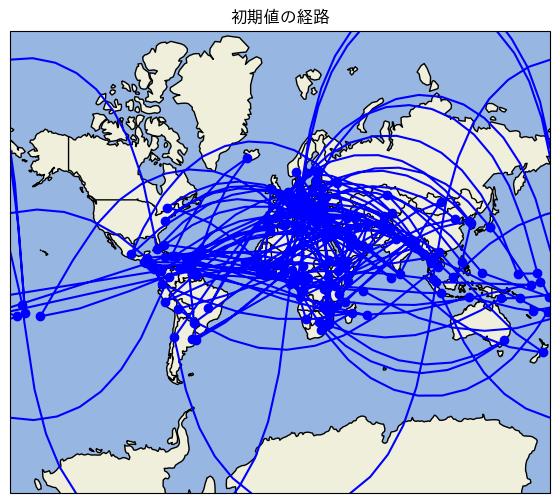
\includegraphics[scale=0.7]{img/init_root.png}
    \end{center}
\end{figure}
URL:\url{https://belka-247d8560.github.io/StochasticAnalysis/template/init_root}

\subsection{温度関数の比較}
摂動は、経路から2都市をランダムに選び、その2都市を入れ替える方法を使用した。この際、異なる温度関数によって結果がどのように変化するかを観察した。\\
\begin{table}[H]
    \centering
    \caption{焼きなまし法を100回行った結果}
    \label{tab:hogehoge}
    \begin{tabular}{ccc}
        温度関数 & 平均結果 & 最小の距離\\
        $e^{-t}$ & 463132.01444166445 & 406531.4913191385\\
        $\frac{1}{\log{(t+2)}}$ & 462349.9561414368 & 394556.62172458577
    \end{tabular}
\end{table}
焼きなまし法を各温度関数で100回ずつ実行した結果が表1に示されている。この結果から、今回の条件では温度関数によって劇的な結果の改善が見られないことがわかった。

\begin{figure}[H]
    \begin{center}
        \includegraphics[scale=0.7]{img/e^{-t}.png}
    \end{center}
\end{figure}
URL:\url{https://belka-247d8560.github.io/StochasticAnalysis/template/temp1}
\begin{figure}[H]
    \begin{center}
        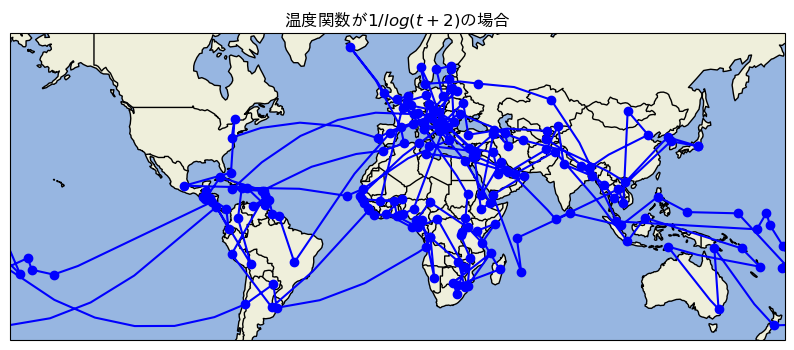
\includegraphics[scale=0.7]{img/log(t+2).png}
    \end{center}
\end{figure}
URL:/\url{https://belka-247d8560.github.io/StochasticAnalysis/template/temp2}

\clearpage
\section{摂動の比較}
次に、摂動の選び方による結果の違いを検証した。温度関数としては $e^{-t}$ を使用した。
摂動の選び方として以下の3つを用いた。
\begin{enumerate}
    \item 2都市をランダムに選び、位置を入れ替える。
    \item 都市とインデックスをランダムに選び、都市をインデックスに挿入する。
    \item 2都市をランダムに選び、その間の順路を逆順にする。
\end{enumerate}

\begin{table}[H]
    \centering
    \caption{焼きなまし法を100回行った結果}
    \label{tab:hogehoge}
    \begin{tabular}{c|c|c|c|}
        摂動 & 平均結果 & 最小の距離 & 摂動回数\\
        1の方法& 460294.3393812061 & 397143.37396547245 & 40418\\
        2の方法 & 438229.86759620294 & 360077.7264521412 & 52523\\
        3の方法 & 263529.5690601708 & 244654.73533840023 & 75053
    \end{tabular}
\end{table}

摂動の選び方による結果の違いを検証した結果、以下のような傾向が確認された。\\
{\bf 1の方法の場合}\\
この方法では、最小距離も他の方法に比べて大きく、探索の効率がやや低いことが示唆される。\\
{\bf 2の方法の場合}\\
この方法では、摂動による改善が比較的効果的であり、平均距離と最小距離の両方が方法1よりも短縮されている。摂動回数も多いため、より広範囲に探索が行われたと考えられる。\\
{\bf 3の方法の場合}\\
この方法では、最も大きな改善が見られ、平均距離と最小距離がいずれも他の方法に比べて大幅に短縮されている。摂動回数も最も多く、探索が効果的に行われたことがわかる。\\

総じて、3つの摂動方法の中では「方法3: 2都市間の順路を逆順にする」が最も効果的であり、他の方法と比べて顕著に短い経路を見つけることができた。この結果から、摂動の選び方が焼きなまし法の性能に大きく影響することが確認できた。
\begin{figure}[H]
    \begin{center}
        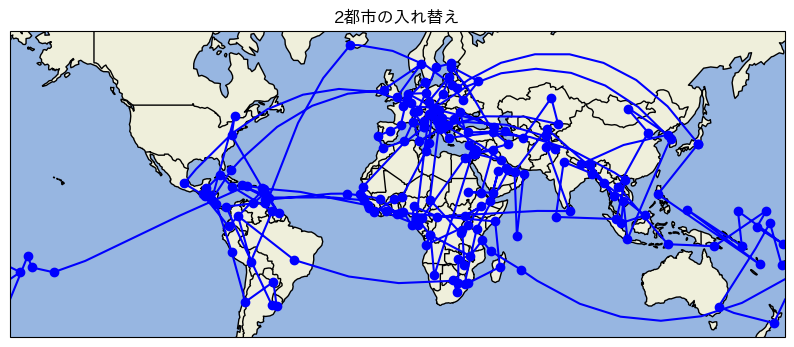
\includegraphics[scale=0.7]{img/two-city-swap.png}
    \end{center}
\end{figure}
URL:\url{https://belka-247d8560.github.io/StochasticAnalysis/template/two-city-swap}
\begin{figure}[H]
    \begin{center}
        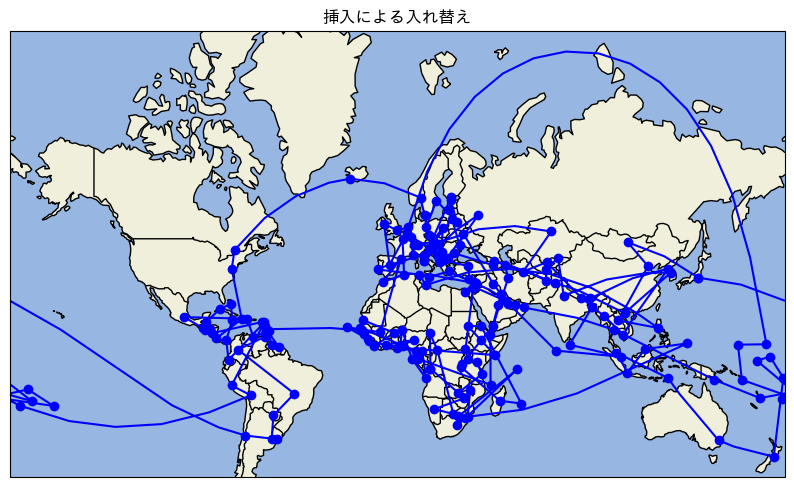
\includegraphics[scale=0.7]{img/insert-swap.png}
    \end{center}
\end{figure}
URL:\url{https://belka-247d8560.github.io/StochasticAnalysis/template/insert-swap}
\begin{figure}[H]
    \begin{center}
        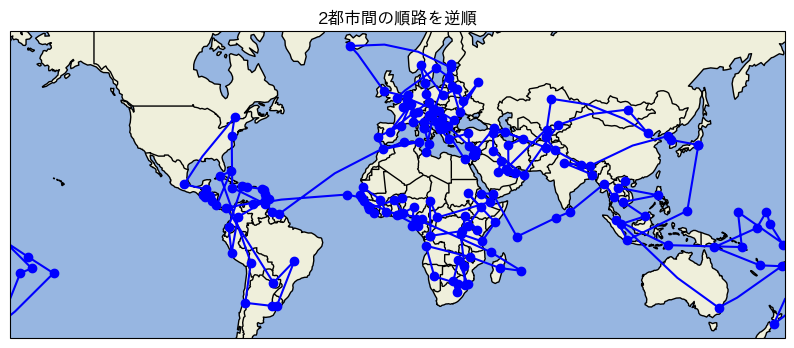
\includegraphics[scale=0.7]{img/two-city-reverse.png}
    \end{center}
\end{figure}
URL:\url{https://belka-247d8560.github.io/StochasticAnalysis/template/two-city-reverse}

\clearpage
\section{付録}
以下に今回使用したコードの全体を記載する。コードは\url{https://github.com/Belka-247d8560/StochasticAnalysis}にも掲載している。
\begin{lstlisting}
"""
### ライブラリをインポートする上での注意  
手元のPython環境次第ではインポートに失敗することがあります。その際はターミナルで
```
pip install -r requirements.txt
```
と試してください。
"""

# 必要なライブラリのインポート
import pandas as pd
import chardet
import numpy as np
import math
import random
from tqdm import tqdm
from time import time
import matplotlib.pyplot as plt
import japanize_matplotlib
import plotly.graph_objs as go
import plotly.io as pio
import cartopy.crs as ccrs
import cartopy.feature as cfeature

#データの読み込み
file_path = "capital_cities_2024.csv"

with open(file_path, 'rb') as f:
    result = chardet.detect(f.read())

encoding = result['encoding']
df = pd.read_csv(file_path, encoding=encoding)
df = df[["ja_ctry", "x", "y"]]
df = df.rename(columns={"ja_ctry":"国", "x":"lon", "y":"lat"})
#国・地域名をリストとして取得
Countries = df["国"].to_list()
#日本スタート、日本終了のリストにする。
Countries.remove('日本国')
Countries = ['日本国'] + Countries + ['日本国']
#緯度、経度を辞書として保存(コードの書きやすさのため)
lat, lon = dict(), dict()
for index, row in df.iterrows():
    lat[row["国"]] = np.radians(row["lat"])
    lon[row["国"]] = np.radians(row["lon"])

#球面三角法の定義
def spherical_trigonometry(lat_p, lon_p, lat_q, lon_q):
    res = np.sin(lat_p) * np.sin(lat_q) + np.cos(lat_p) * np.cos(lat_q) * np.cos(lon_q - lon_p)
    res = np.arccos(res)
    R = 6378 # 地球の半径 (km)
    res *= R
    
    return res

#総距離の計算関数の定義
def calculating_the_total_distance(Countries_list):
    N = len(Countries_list)
    res = 0
    for i in range(N-1):
        now_country, next_country = Countries_list[i], Countries_list[i+1]
        res += spherical_trigonometry(lat[now_country], lon[now_country], lat[next_country], lon[next_country])
    return res

#メルカトル図法での結果の描画
def mercator_plot(Countries_list, filename):
    lats = [np.degrees(lat[Country]) for Country in Countries_list]
    lons = [np.degrees(lon[Country]) for Country in Countries_list]
    plt.figure(figsize=(10, 6))
    ax = plt.axes(projection=ccrs.Mercator())
    ax.add_feature(cfeature.COASTLINE)
    ax.add_feature(cfeature.BORDERS)
    ax.add_feature(cfeature.LAND)
    ax.add_feature(cfeature.OCEAN)
    plt.plot(lons, lats, marker='o', linestyle='-', color='b', transform=ccrs.Geodetic())
    plt.xlabel("経度")
    plt.ylabel("緯度")
    plt.title(filename)
    plt.grid(True)
    plt.show()

#地球儀上への結果の描画
def globe_plot(Countries_list, filename=None):
    lats = [df.loc[df['国']==Country, 'lat'].values[0] for Country in Countries_list]
    lons = [df.loc[df['国']==Country, 'lon'].values[0] for Country in Countries_list]

    line = go.Scattergeo(
        lon=lons,
        lat=lats,
        mode='lines+markers',
        line=dict(color='yellow', width=2),
        marker=dict(size=8, color='red')
    )

    layout = go.Layout(
        geo=dict(
            projection=dict(type='orthographic'),
            showcountries=True,
        ),
        margin=dict(r=10, l=10, b=10, t=10)
    )

    fig = go.Figure(data=[line], layout=layout)
    pio.show(fig)
    
    if filename:
        pio.write_html(fig, file = filename)

#初期値の総距離の計算、描画
print("初期値:", *Countries)
print("総距離:", calculating_the_total_distance(Countries), "km")
# メルカトル図法での初期値の描画
mercator_plot(Countries, '初期値の経路')
# 地球儀上への初期値の描画
globe_plot(Countries, 'init_root')

# 温度関数による結果の比較
#温度関数の定義
def cooling_function1(init_temp, end_temp, start_time, max_time):
    T_max = math.exp(0)
    T_min  = math.exp(-max_time)
    T = math.exp(-(time() - start_time))
    res = end_temp  + (init_temp - end_temp)*((T - T_min) / (T_max - T_min))
    return res
def cooling_function2(init_temp, end_temp, start_time, max_time):
    T_max = 1/math.log(2)
    T_min  = 1/math.log(max_time + 2)
    T = 1/math.log((time() - start_time) + 2)
    res = end_temp  + (init_temp - end_temp)*((T - T_min) / (T_max - T_min))
    return res
    
#評価関数
def cost_function(x, y, Countries_list):
    now_cost, next_cost = 0, 0
    x_pre_country, x_country, x_next_country = Countries_list[x-1:x+2]
    y_pre_country, y_country, y_next_country = Countries_list[y-1:y+2]
    now_cost = spherical_trigonometry(lat[x_pre_country], lon[x_pre_country], lat[x_country], lon[x_country])\
            + spherical_trigonometry(lat[x_country], lon[x_country], lat[x_next_country], lon[x_next_country])\
            + spherical_trigonometry(lat[y_pre_country], lon[y_pre_country], lat[y_country], lon[y_country])\
            + spherical_trigonometry(lat[y_country], lon[y_country], lat[y_next_country], lon[y_next_country])
    next_cost = spherical_trigonometry(lat[x_pre_country], lon[x_pre_country], lat[y_country], lon[y_country])\
            + spherical_trigonometry(lat[y_country], lon[y_country], lat[x_next_country], lon[x_next_country])\
            + spherical_trigonometry(lat[y_pre_country], lon[y_pre_country], lat[x_country], lon[x_country])\
            + spherical_trigonometry(lat[x_country], lon[x_country], lat[y_next_country], lon[y_next_country])
    return now_cost, next_cost

#焼きなまし法
def simulated_annealing(Countries_list, cooling_function, cost_function, init_temp, end_temp, start_time, max_time):
    T = init_temp
    while time() - start_time <= max_time:
        a, b = random.choices(range(1, len(Countries_list)-1), k=2)
        now_cost, next_cost = cost_function(a, b, Countries_list)
        if next_cost < now_cost or random.random() < np.exp(-np.abs(now_cost - next_cost)/T):
            Countries_list[a], Countries_list[b] = Countries_list[b], Countries_list[a]
        T = cooling_function(init_temp, end_temp, start_time, max_time)
    return Countries_list

#1つ目の温度関数で焼きなまし法を100回行う
min_result = []
min_distance = float('inf')
average_distance = 0
for i in tqdm(range(100)):
    result = simulated_annealing(Countries_list=Countries.copy(), cooling_function=cooling_function1, cost_function=cost_function, init_temp=10000, end_temp=0.001, start_time=time(), max_time=2)
    distance = calculating_the_total_distance(result)
    if distance < min_distance:
        min_distance = distance
        min_result = result.copy()
    average_distance += distance
print("最小の距離:", min_distance)
print("最小の距離での巡回順番:", *min_result)
print("平均:", average_distance/100)

# メルカトル図法での最小の結果の描画
mercator_plot(min_result, '温度関数が$e^{-t}$の場合')
# 地球儀上への最小の結果の描画
globe_plot(Countries, 'temp1')

#2つ目の温度関数で焼きなまし法を100回行う
min_result = []
min_distance = float('inf')
average_distance = 0
for i in tqdm(range(100)):
    result = simulated_annealing(Countries_list=Countries.copy(), cooling_function=cooling_function2, cost_function=cost_function, init_temp=10000, end_temp=0.001, start_time=time(), max_time=2)
    distance = calculating_the_total_distance(result)
    if distance < min_distance:
        min_distance = distance
        min_result = result.copy()
    average_distance += distance
print("最小の距離:", min_distance)
print("最小の距離での巡回順番:", *min_result)
print("平均:", average_distance/100)

# メルカトル図法での最小の結果の描画
mercator_plot(min_result, '温度関数が$1/log(t+2)$の場合')
# 地球儀上への最小の結果の描画
globe_plot(Countries, 'temp2')

# 摂動による結果の比較
def cooling_function(init_temp, end_temp, start_time, max_time):
    T_max = math.exp(0)
    T_min  = math.exp(-max_time)
    T = math.exp(-(time() - start_time))
    res = end_temp  + (init_temp - end_temp)*((T - T_min) / (T_max - T_min))
    return res

### 2都市をランダムに選び、入れ替える方法の場合
def cost_function(x, y, Countries_list):
    now_cost, next_cost = 0, 0
    x_pre_country, x_country, x_next_country = Countries_list[x-1:x+2]
    y_pre_country, y_country, y_next_country = Countries_list[y-1:y+2]
    now_cost = spherical_trigonometry(lat[x_pre_country], lon[x_pre_country], lat[x_country], lon[x_country])\
            + spherical_trigonometry(lat[x_country], lon[x_country], lat[x_next_country], lon[x_next_country])\
            + spherical_trigonometry(lat[y_pre_country], lon[y_pre_country], lat[y_country], lon[y_country])\
            + spherical_trigonometry(lat[y_country], lon[y_country], lat[y_next_country], lon[y_next_country])
    next_cost = spherical_trigonometry(lat[x_pre_country], lon[x_pre_country], lat[y_country], lon[y_country])\
            + spherical_trigonometry(lat[y_country], lon[y_country], lat[x_next_country], lon[x_next_country])\
            + spherical_trigonometry(lat[y_pre_country], lon[y_pre_country], lat[x_country], lon[x_country])\
            + spherical_trigonometry(lat[x_country], lon[x_country], lat[y_next_country], lon[y_next_country])
    return now_cost, next_cost

def simulated_annealing(Countries_list, cooling_function, cost_function, init_temp, end_temp, start_time, max_time):
    T = init_temp
    # cnt = 0
    while time() - start_time <= max_time:
        # cnt += 1
        a, b = random.choices(range(1, len(Countries_list)-1), k=2)
        now_cost, next_cost = cost_function(a, b, Countries_list)
        if next_cost < now_cost or random.random() < np.exp(-np.abs(now_cost - next_cost)/T):
            Countries_list[a], Countries_list[b] = Countries_list[b], Countries_list[a]
        T = cooling_function(init_temp, end_temp, start_time, max_time)
    # print('摂動回数:', cnt)
    return Countries_list

#焼きなまし法を100回行う
min_result = []
min_distance = float('inf')
average_distance = 0
for i in tqdm(range(100)):
    result = simulated_annealing(Countries_list=Countries.copy(), cooling_function=cooling_function, cost_function=cost_function, init_temp=10000, end_temp=0.001, start_time=time(), max_time=2)
    distance = calculating_the_total_distance(result)
    if distance < min_distance:
        min_distance = distance
        min_result = result.copy()
    average_distance += distance
print("最小の距離:", min_distance)
print("最小の距離での巡回順番:", *min_result)
print("平均:", average_distance/100)

# メルカトル図法での最小の結果の描画
mercator_plot(min_result, '2都市の入れ替え')
# 地球儀上への最小の結果の描画
globe_plot(Countries, 'two-city-swap')

# 挿入での方法の場合
def cost_function(x, y, Countries_list):
    now_cost, next_cost = 0, 0
    x_pre_country, x_country, x_next_country = Countries_list[x-1:x+2]
    y_pre_country, y_next_country = Countries_list[y:y+2]
    now_cost = spherical_trigonometry(lat[x_pre_country], lon[x_pre_country], lat[x_country], lon[x_country])\
            + spherical_trigonometry(lat[x_country], lon[x_country], lat[x_next_country], lon[x_next_country])\
            + spherical_trigonometry(lat[y_pre_country], lon[y_pre_country], lat[y_next_country], lon[y_next_country])
    Countries_list.pop(x)
    Countries_list.insert(y, x_country)
    next_cost = spherical_trigonometry(lat[x_pre_country], lon[x_pre_country], lat[x_next_country], lon[x_next_country])\
            + spherical_trigonometry(lat[y_pre_country], lon[y_pre_country], lat[x_country], lon[x_country])\
            + spherical_trigonometry(lat[x_country], lon[x_country], lat[y_next_country], lon[y_next_country])
    return now_cost, next_cost

def simulated_annealing(Countries_list, cooling_function, cost_function, init_temp, end_temp, start_time, max_time):
    T = init_temp
    # cnt = 0
    while time() - start_time <= max_time:
        # cnt += 1
        a, b = random.choices(range(1, len(Countries_list)-1), k=2)
        now_cost, next_cost = cost_function(a, b, Countries_list)
        if not (next_cost < now_cost or random.random() < np.exp(-np.abs(now_cost - next_cost)/T)):
            Country = Countries_list.pop(b)
            Countries_list.insert(a, Country)
        T = cooling_function(init_temp, end_temp, start_time, max_time)
    # print('摂動回数:', cnt)
    return Countries_list

#焼きなまし法を100回行う
min_result = []
min_distance = float('inf')
average_distance = 0
for i in tqdm(range(100)):
    result = simulated_annealing(Countries_list=Countries.copy(), cooling_function=cooling_function, cost_function=cost_function, init_temp=10000, end_temp=0.001, start_time=time(), max_time=2)
    distance = calculating_the_total_distance(result)
    if distance < min_distance:
        min_distance = distance
        min_result = result.copy()
    average_distance += distance
print("最小の距離:", min_distance)
print("最小の距離での巡回順番:", *min_result)
print("平均:", average_distance/100)

# メルカトル図法での最小の結果の描画
mercator_plot(min_result, '挿入による入れ替え')
# 地球儀上への最小の結果の描画
globe_plot(Countries, 'insert-swap')

# 順路を逆順にする方法の場合
def cost_function(x, y, Countries_list):
    now_cost, next_cost = 0, 0
    x_pre_country, x_country = Countries_list[x-1:x+1]
    y_country, y_next_country = Countries_list[y:y+2]
    now_cost = spherical_trigonometry(lat[x_pre_country], lon[x_pre_country], lat[x_country], lon[x_country])\
            + spherical_trigonometry(lat[y_country], lon[y_country], lat[y_next_country], lon[y_next_country])
    next_cost = spherical_trigonometry(lat[x_pre_country], lon[x_pre_country], lat[y_country], lon[y_country])\
            + spherical_trigonometry(lat[x_country], lon[x_country], lat[y_next_country], lon[y_next_country])
    return now_cost, next_cost

def simulated_annealing(Countries_list, cooling_function, cost_function, init_temp, end_temp, start_time, max_time):
    T = init_temp
    # cnt = 0
    while time() - start_time <= max_time:
        # cnt += 1
        a, b = random.choices(range(1, len(Countries_list)-1), k=2)
        now_cost, next_cost = cost_function(a, b, Countries_list)
        if next_cost < now_cost or random.random() < np.exp(-np.abs(now_cost - next_cost)/T):
            Countries_list[a:b+1] = Countries_list[a:b+1][::-1]
        T = cooling_function(init_temp, end_temp, start_time, max_time)
    # print('摂動回数:', cnt)
    return Countries_list

#焼きなまし法を100回行う
min_result = []
min_distance = float('inf')
average_distance = 0
for i in tqdm(range(100)):
    result = simulated_annealing(Countries_list=Countries.copy(), cooling_function=cooling_function, cost_function=cost_function, init_temp=10000, end_temp=0.001, start_time=time(), max_time=2)
    distance = calculating_the_total_distance(result)
    if distance < min_distance:
        min_distance = distance
        min_result = result.copy()
    average_distance += distance
print("最小の距離:", min_distance)
print("最小の距離での巡回順番:", *min_result)
print("平均:", average_distance/100)

# メルカトル図法での最小の結果の描画
mercator_plot(min_result, '2都市間の順路を逆順')
# 地球儀上への最小の結果の描画
globe_plot(Countries, 'two-city-reverse')
\end{lstlisting}
\end{document}